\documentclass[a4paper]{article}

% Use the postscript times font!
\usepackage{times}
\usepackage{soul}
\usepackage[hyphens]{url}
\usepackage[hidelinks]{hyperref}
\usepackage[utf8]{inputenc}
\usepackage[small]{caption}
\usepackage{graphicx}
\usepackage{subcaption}
\usepackage{amsmath,amssymb}
\usepackage{booktabs}
\usepackage[a4paper, portrait, margin=1in]{geometry}
\urlstyle{same}

\usepackage{parskip}

% the following package is optional:
%\usepackage{latexsym} 

\title{
\includegraphics[scale=0.75]{images/unblogo.jpg}\\CS6735 Programming Project Report}

\makeatletter
\renewcommand\@date{{%
  \vspace{-\baselineskip}%
  \large\centering
  \begin{tabular}{@{}c@{}}
    Ethan Garnier\textsuperscript{1} \\
    \normalsize ethan.garnier78@unb.ca 
  \end{tabular}%
  \hspace{3mm}
  \begin{tabular}{@{}c@{}}
    Matthew Tidd\textsuperscript{2} \\
    \normalsize mtidd2@unb.ca
  \end{tabular}
  \hspace{3mm}
  \begin{tabular}{@{}c@{}}
    Minh Nguyen\textsuperscript{2} \\
    \normalsize mnguyen6@unb.ca
  \end{tabular}
  
  \bigskip

  \textsuperscript{1}Department of Electrical and Computer Engineering, UNB\par
  \textsuperscript{2}Department of Mechanical Engineering, UNB

  \bigskip

  \today
}}
\makeatother

\begin{document}

\maketitle

\begin{abstract}
    TODO
\end{abstract}

\newpage

\section{Introduction}

\section{Adaboost with ID3 Base Learner}
The Adaptive Boosting (Adaboost) classification algorithm was successfully implemented using the Python 3 programming language. The version of Adaboost implemented used the Iterative Dichotomiser 3 (ID3) decision tree learning algorithm as a weak learner. This algorithm was trained on a dataset of English alphabet character image features and used to identify letters of the alphabet based on these features, i.e., letter recognition.

\subsection{Adaboost}
Adaboost is a boosted classifier that uses multiple weak hypotheses to build a single, strong hypothesis to be used for classification. These weak hypotheses are initially learned through a weak base learner algorithm, with the performance of these weak hypotheses dictating their weight in the final, strong hypothesis. To accomplish this, Adaboost first assigns an initial weight of $1/N$ to every training example, where $N$ is the number of training examples. Upon training of a weak hypothesis, Adaboost sums the weight of all misclassified examples against the trained weak hypothesis.  This sum, called the $error$ or $\epsilon$, is used to calculate the weight, or $\alpha$, for the given weak hypothesis according to Equation~\ref{eq:weak-h-alpha}.

\begin{equation}
    \label{eq:weak-h-alpha}
    \alpha = \frac{1}{2}\ln\left(\frac{1-\epsilon}{\epsilon}\right)
\end{equation}

This process of training weak learners and calculating the $\alpha$ of those weak learners is repeated $T$ times. On each iteration of the boosting algorithm, $t \le T$, the weights of all $N$ training examples for the next iteration, $w_{i, t+1}$, are updated according to Equation~\ref{eq:example-weight-update}.

\begin{equation}
    \label{eq:example-weight-update}
    w_{i, t+1} =
    \begin{cases} 
      w_{i,t}e^{-\alpha_t} & h_t(x_i) = y_i \\
      w_{i,t}e^{\alpha_t} & h_t(x_i) \ne y_i \\
   \end{cases}
\end{equation}

Where $w_{i,t}$ is the weight of training example $i$ for the current iteration, $\alpha_t$ is the weight of the most recently learned weak hypothesis, $h_t(x_i)$ is the classification of training example $i$ using this weak hypothesis, and $y_i$ is the correct classification of example $i$. These newly calculated weights are then normalized to ensure the sum of all training example weights is one. As can be seen from Equation~\ref{eq:example-weight-update}, the weight of incorrectly classified training examples is increased, whereas correctly classified examples have their weights decreased. The reason for this is that Adaboost wants the weak base learners to place extra emphasis on learning the incorrectly classified examples to produce a more accurate result in the end. Details on how this is executed lies within the chosen weak base learner algorithm. 

\subsection{ID3}
For this implementation of Adaboost, the ID3 algorithm was chosen as the weak base learner. ID3 is a greedy, recursive learning algorithm that generates binary decision trees from a given dataset, \textit{S}, where each internal node represents a feature by which \textit{S} is split, and leaf nodes represent a classification for the remaining examples in \textit{S}. The inductive bias of the ID3 algorithm is that it prefers shorter decision trees, building off the idea that a short hypothesis that fits the data well is unlikely to be a coincidence, as opposed to a larger hypothesis. This bias of the ID3 algorithm is enforced through its statistically based splitting criteria. At each internal node, the entropy of the dataset \textit{S} is calculated based on Equation~\ref{eq:entropy}.

\begin{equation}
    \label{eq:entropy}
    Entropy(S) = -\sum_{x \in X} p(x)log(p(x))
\end{equation}

Where $X$ is the set of all classifications in $S$, and $p(x)$ is the probability of a given classification in $S$. Once the entropy for $S$ is calculated, every attribute value for every attribute in $S$ is examined as a potential split attribute value. This is done by calculating the information gain of splitting $S$ based on that attribute value according to Equation~\ref{eq:info-gain}.

\begin{equation}
    \label{eq:info-gain}
    Gain(S, A, V) = Entropy(S) - \left(\frac{|S_{\le V}|}{|S|}\times Entropy(S_{\le V}) + \frac{|S_{> V}|}{|S|}\times Entropy(S_{> V}) \right)
\end{equation}

Where $S_{\le V}$ is the subset of training examples in $S$ whose value for attribute $A$ is less than or equal to $V$, and $S_{> V}$ is the subset of training examples in $S$ whose value for attribute $A$ is greater than $V$. The largest information gain calculated for the current internal node determines the feature and feature value by which the data will be split going to the next level of the decision tree. The fact that there are only two splits for each internal node shows that this is a binary decision tree. This splitting of training examples and building of binary decision tree continues until one of the given three base cases are met:
\begin{enumerate}
    \item Base Case 1 - Every training example in \textit{S} belong to the same class. If this is the case, then return that class.

    \item Base Case 2 - There are no remaining attributes to split the data off of. If this is the case, then return the class of majority for the training examples in \textit{S}.

    \item Base Case 3 - There are no training examples in \textit{S}. If this is the case, then return the class of majority for the training examples of the parent node.
\end{enumerate}
Base case 3 is especially important, as it is this which provides the ID3 algorithm with its generalizing power. A slight change to the ID3 algorithm was made in this implementation to account for it being used as a weak base learner in Adaboost. As previously mentioned, Adaboost will update the weights of each training example over its iterations to favor the incorrectly classified examples. The weak base learner, ID3 in this case, must therefore take these weights into account to try extra hard to correctly learn these incorrectly classified examples. This was accomplished by modifying Equation~\ref{eq:info-gain} to account for the total weight of the example subsets. This can be seen in Equation~\ref{eq:weighted-info-gain}.

\begin{equation}
    \label{eq:weighted-info-gain}
    Gain(S, A, V) = Entropy(S) - \left(\frac{\sum_{e \in S_{\le V}}w_e}{|S|}\times Entropy(S_{\le V}) + \frac{\sum_{e \in S_{> V}}w_e}{|S|}\times Entropy(S_{> V}) \right)
\end{equation}

\subsection{Predicting with Adaboost}
Once the $T$ weak hypotheses have been trained and each has their own associated weight $\alpha_t$, it is time to begin classifying test data. For each testing example $x_i$, $T$ classifications are acquired by classifying that example with each of the trained weak hypothesis. For each unique classification of $x_i$, the weights, or $\alpha_t$, of all base hypotheses that gave that classification are summed and this sum represents the weight of this classification for $x_i$. The classification with the largest weight becomes the final, or returned classification for testing example $x_i$. This process is repeated for all testing examples.

\subsection{Implementation Details}
This section will outline all details related to this implementation of Adaboost and the ID3 algorithm.

\subsubsection{Development Platform and Libraries}
As was previously mentioned, all code written to implement the Adaboost and ID3 algorithms was written in Python 3. This code was written to run on a Windows operation system, but will run on any system that can run the Python programming language. All development was conducted through the Visual Studios Code text editor, and code versioning was controlled through Git to a remote repository hosted on GitHub. The Adaboost and ID3 algorithms were written completely from scratch using only Python's built-in functions, the \textit{Numpy} Python library for mathematical operations, and the \textit{Pandas} Python library for data manipulation and representation. The \textit{scikit-learn} maching learning Python library was used for pre-processing of training and testing data, as well as for evaluating the performance of the manually implemented algorithms. This machine learning library was not included or used in any of the Adaboost or ID3 algorithm implementations.

\subsubsection{Program Structure}
Python classes were used to structure the various components of this Adaboost implementation. These classes included: \textit{AdaBoost} (adaboost.py), \textit{ID3Classifier} (id3.py), and \textit{BinaryDecisionTree} (tree.py). By following an object oriented approach, different instances of the learning algorithms could be instantiated with different hyper-parameters and then re-used when needed. This, in addition to allowing these classes to keep track of their own internal state while training, significantly cleaned up and optimized the code. For example, the \textit{AdaBoost} class has it's own internal member variables named \textit{models} and \textit{alphas} which store the trained weak hypotheses and their corresponding weights, respectively. This means that once the \textit{AdaBoost} models have been trained, these models and their weights can easily be accessed through these member variables, vastly reducing the amount of code required to keep track of this state. In addition to this, the \textit{ID3Classifier} class contains two private static methods used to calculate the entropy and information gain throughout its training process.

\subsubsection{Data-Structures}
The Dataframe data structure, as part of the \textit{Pandas} library, is a data structure that allows for data to be represented in a two-dimensional tabular format and was used extensively throughout this project. Using Dataframes allowed for the training and testing data to easily be extracted, segmented, manipulated, and represented throughout the entire training and classification process. Although operations on Dataframes are extremely slow, they also allow for the data to be exported to a two-dimensional Numpy array, and this feature was used a lot for data manipulation and calculations. Finally, Dataframes were leveraged to store training and classification results of the Adaboost algorithm in a tabular format and to export these results to a .csv file.

A binary tree data structure was manually implemented in Python to fulfill the decision tree output of the ID3 algorithm. This binary tree implementation, named \textit{BinaryDecisionTree} in tree.py, is a recursive tree data structure that possesses four attributes: 1) a split feature index, 2) a split feature value, 3) a truth branch, 4) a false branch. The split feature index of the \textit{BinaryDecisionTree} is an integer value that represents the feature this node splits on in the training data. Instead of storing the name of the feature as a string, the index of the feature in the list of feature names is stored. This is done to improve performance. The split feature value is exactly as the name describes, it is the value of the split feature by which this node splits the data on. The truth branch is a reference to another \textit{BinaryDecisionTree} object, hence the recursive nature of the data structure. When traversing the \textit{BinaryDecisionTree}, this branch is evaluated when a provided feature value is greater than the split feature value of this node. Finally, the false branch is a reference to another \textit{BinaryDecisionTree} object that is evaluated when a provided feature value is less than or equal to the split feature value of this node. The form of the trees built by the \textit{BinaryDecisionTree} object can be seen in Figure~\ref{fig:binary-decision-tree}. 

\begin{figure}[h]
    \centering
    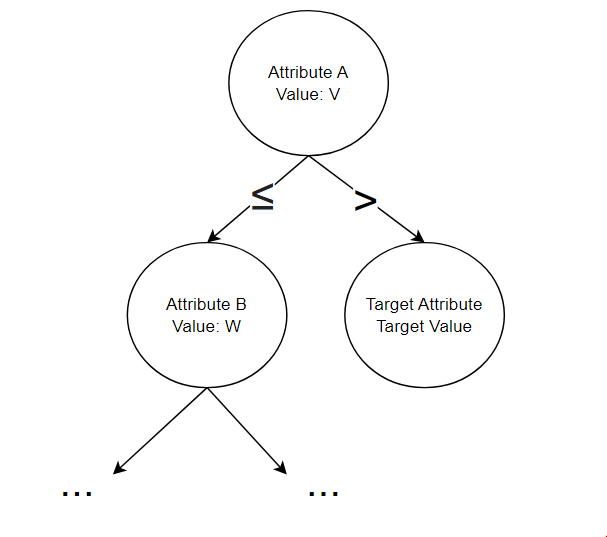
\includegraphics[scale=0.55]{images/binary-decision-tree.PNG}
    \caption{Binary decision tree created by \textit{BinaryDecisionTree} class.}
    \label{fig:binary-decision-tree}
\end{figure}

As can be seen in Figure~\ref{fig:binary-decision-tree}, leaf nodes of the tree generated by \textit{BinaryDecisionTree} have their split feature set to the target attribute of the data set, and the split feature value is the classification of the target attribute. The true and false branches are empty. As such, predictions can be made on a learned \textit{BinaryDecisionTree} for a given testing example by simply following the trees branches, checking the testing example's feature values with the split feature values at each node, until a leaf is reached where the classification for the testing example is returned.

\subsubsection{Algorithm Hyper-Parameters}
Two hyper-parameters were implemented for this Adaboost with ID3 base learner implementation. These hyper-parameters include: 1) the maximum tree depth of the learned binary decision trees, and 2) the number of weak hypotheses learned by Adaboost. 

The maximum tree depth of the learned binary decision tree is a hyper-parameter of the ID3 algorithm implementation, and it sets a limit on the maximum depth of recursion of the algorithm. This depth was monitored as a \textit{depth} parameter incremented on each recursive call. When the maximum depth was reached, the target value of majority in the current data set was returned as the leaf node. If the caller did not specify a maximum tree depth, then a tree depth of infinity was set, which essentially means the algorithm would only return a leaf node if one of its original three base cases were hit. It was experimentally determined, as can be seen in Figure~\ref{fig:depth-hyper-param}, that placing a limit on the depth of the trained binary decision tree less than the number of features in the data set actually reduces classification accuracy. For context, Figure~\ref{fig:depth-hyper-param} used a dataset with 16 features. This makes intuitive sense, as each node splits on a single feature, so there can only ever be a tree as deep as the number of features. Also, if we force a tree to terminate early, then we are forcing it to over generalize the data. Either way, this hyper-parameter remained as reducing the depth of the tree significantly improves training and classification performance. 

\begin{figure}[h]
    \centering
    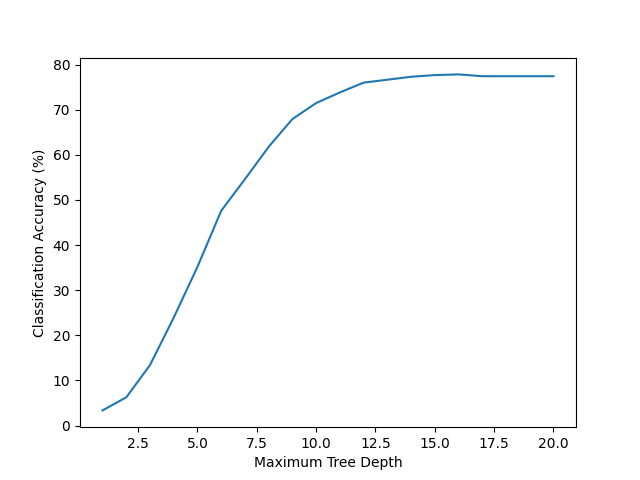
\includegraphics[scale=0.7]{images/tree-depth-plot.png}
    \caption{Accuracy of classification vs. maximum tree depth of learned binary decision tree by ID3 algorithm.}
    \label{fig:depth-hyper-param}
\end{figure}

The second hyper-parameter implemented, the number of weak hypotheses learned by the Adaboost algorithm, is a hyper-parameter of the Adaboost algorithm that controls the number of models trained by the weak base learner for a single Adaboost training session. This hyper-parameter has direct influence on the performance of the Adaboost algorithm, both from a time point-of-view and an accuracy point-of-view. The more weak hypotheses trained, the longer training will take; however, the more accurate classification can become. It was experimentally determined that 14 is the optimal number of weak hypotheses to learn as it maximizes the classification accuracy while keeping the training time as low as possible. Figure~\ref{fig:estimator-hyper-param} demonstrates how at 14 weak hypotheses, the classification accuracy of the Adaboost algorithm reaches an asymptote. Although this is only for a particular split of the dataset, it remains consistent. Figure~\ref{fig:estimator-time} shows how the time taken for training the Adaboost algorithm increases linearly with the number of weak hypotheses learned by the algorithm. As such, it is optimal to use 14 weak hypotheses to maximize classification accuracy while ensuring training time doesn't continue to increase.

\begin{figure}[h]
    \centering
    \begin{subfigure}[t]{0.48\textwidth}
        \centering
        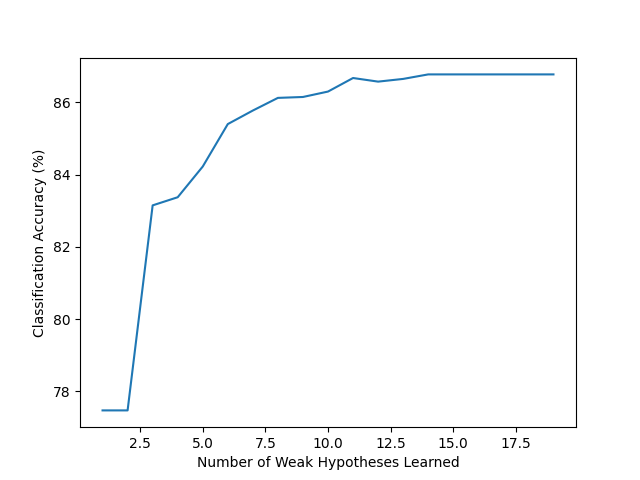
\includegraphics[width=\linewidth]{images/n-weak-hypotheses-plot.png}
        \caption{}
        \label{fig:estimator-hyper-param}
    \end{subfigure}%
    ~ 
    \begin{subfigure}[t]{0.48\textwidth}
        \centering
        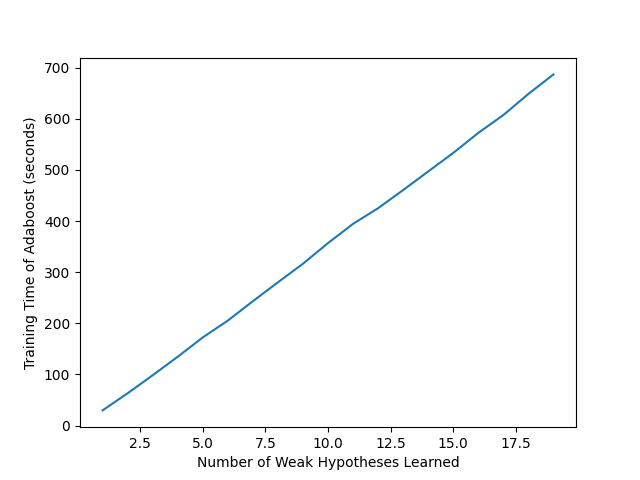
\includegraphics[width=\linewidth]{images/adaboost-training-time.png}
        \caption{}
        \label{fig:estimator-time}
    \end{subfigure}

    \caption{Performance of the number of weak hypotheses trained by Adaboost algorithm during training vs. (a) classification accuracy, and (b) time taken to train the model.}
    \label{fig:adaboost-hyper-param}
\end{figure}   

\subsection{Dataset Details}
This section will outline all details related to dataset used to train and test the Adaboost implementation. 

\subsubsection{Description of Dataset}
The dataset was taken from the UC Irvine Machine Learning Repository and has the ID 59 within this repository. The goal of the dataset is to identify each entry as a capital letter from the English alphabet based on 16 primitive numerical attributes extracted from a black-and-white image of the letter that the entry represents. The dataset contains 20 thousand entries with 17 columns for each entry, 16 columns being the previously mentioned primitive numerical attributes, and the final column being the classification of the entry, a letter in this case. These 16 primitive numerical attributes, or features in the context of machine learning, are integer values between 0 and 15 and are described as the following:
\begin{enumerate}
    \item x-box - Horizontal position of box.
    \item y-box - Vertical position of box.
    \item width - Width of box.
    \item hight - Height of box.
    \item onpix - Total number on pixels.
    \item x-bar - Mean x of on pixels in box.
    \item y-bar - Mean y of on pixels in box.
    \item x2bar - Mean x variance.
    \item y2bar - Mean y variance.
    \item xybar - Mean x y correlation.
    \item x2ybr - Mean of x * x * y.
    \item xy2br - Mean of x * y * y.
    \item x-ege - Mean edge count left to right.
    \item xegvy - Correlation of x-ege with y.
    \item y-ege - Mean edge count bottom to top.
    \item yegvx - Correlation of y-ege with x.
\end{enumerate}

The total number of classes in this dataset is 26, representing the number of capital letters in the English alphabet. The distribution of classes within the dataset is nearly uniform, as can be seen in Figure~\ref{fig:class-histogram}. As such, no re-sampling of data was needed.

\begin{figure}[h]
    \centering
    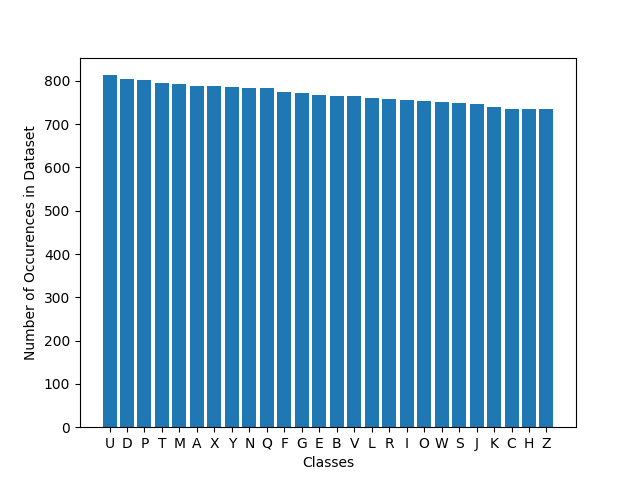
\includegraphics[scale=0.7]{images/class-distribution.png}
    \caption{Distribution of classes within the Letter Distribution dataset.}
    \label{fig:class-histogram}
\end{figure}

\subsubsection{Pre-Processing}
As previously mentioned, there are no missing values within the dataset used. As such, no pre-processing of the data to remove partial entries was required. The only pre-processing performed on the dataset was to split the data into testing and training datasets using the \textit{train\_test\_split()} function from the \textit{scikit-learn} machine learning library. A split of 80\%/20\% (16000/4000) was used for training and testing, respectively, as this was the split suggested by UC Irvine on the dataset's webpage. As such, in all results presented in the next sections, the Adaboost algorithm was trained on 16 000 randomly selected entries, and tested on the remaining 4000 entries of the dataset.

\subsection{Experimental Results}

\section{Conclusion}

\newpage

% Bibliography/Reference Stuff
\bibliographystyle{abbrv}
\bibliography{main}
\end{document}